\documentclass[12pt,a4paper]{article}
\usepackage[utf8]{inputenc}
\usepackage[T1]{fontenc}
\usepackage{amsmath,amssymb,amsfonts}
\usepackage{graphicx}
\usepackage{booktabs}
\usepackage{hyperref}
\usepackage{geometry}
\usepackage{fancyhdr}
\usepackage{tikz}
\usetikzlibrary{shapes,arrows,positioning}

\geometry{margin=1in}
\pagestyle{fancy}
\fancyhf{}
\rhead{Z$^2$ Framework}
\lhead{Dimensional Analysis}
\rfoot{Page \thepage}

\title{\textbf{Dimensional Analysis: An Honest Clarification}\\[0.5em]
\large What ``Dimension'' Actually Means in Different Contexts}
\author{Carl Zimmerman}
\date{May 2026}

\begin{document}

\maketitle

\begin{abstract}
The word ``dimension'' is used in at least five different ways in physics and philosophy: spatial dimensions, spacetime dimensions, compactified dimensions, mathematical dimensions, and perceptual dimensions. These are NOT the same thing. This document provides honest clarification of what each means in the context of the Z$^2$ framework and addresses common confusions about the 7D structure and 8 fixed points.
\end{abstract}

\tableofcontents
\newpage

\section{Why This Document Exists}

The word ``dimension'' is used in at least five different ways:
\begin{enumerate}
\item \textbf{Spatial dimensions} (the room you're in)
\item \textbf{Spacetime dimensions} (physics)
\item \textbf{Compactified dimensions} (extra dimensions in string theory/KK)
\item \textbf{Mathematical dimensions} (abstract spaces)
\item \textbf{Perceptual/phenomenal dimensions} (perspectives of consciousness)
\end{enumerate}

\textbf{These are NOT the same thing.} Conflating them leads to confusion.

\section{The Z$^2$ Orbifold Structure}

\subsection{What We Actually Claim}

The Z$^2$ framework proposes:
\begin{equation}
\text{TOTAL SPACETIME} = M_4 \times T^3/Z_2 = 7 \text{ dimensions}
\end{equation}

\begin{itemize}
\item $M_4$: 4-dimensional Minkowski spacetime $(t, x, y, z)$---this is what you experience directly
\item $T^3/Z_2$: 3-dimensional orbifold $(y^1, y^2, y^3)$---these are COMPACTIFIED at tiny scales; you do NOT directly perceive them
\end{itemize}

\subsection{What ``Compactified'' Means}

Imagine an ant walking on a drinking straw:
\begin{itemize}
\item Along the straw: it can walk far (non-compact, ``large'' dimension)
\item Around the straw: it goes in circles (compact, ``curled up'' dimension)
\end{itemize}

In the Z$^2$ framework:
\begin{itemize}
\item The 4 spacetime dimensions $(t, x, y, z)$: non-compact, infinite extent
\item The 3 internal dimensions ($T^3/Z_2$): compact, radius $R \sim 10^{-35}$ meters
\end{itemize}

\textbf{You cannot ``go to'' the extra dimensions.} They are at every point in space, but curled up smaller than any probe can detect.

\subsection{The 8 Fixed Points}

The $T^3/Z_2$ orbifold has 8 special points where the $Z_2$ identification creates singularities:
\begin{equation}
T^3 = \text{torus with coordinates } (y^1, y^2, y^3) \in [0, 2\pi)^3
\end{equation}
\begin{equation}
Z_2 \text{ action}: (y^1, y^2, y^3) \rightarrow (-y^1, -y^2, -y^3)
\end{equation}

Fixed points: where $y = -y$ (mod $2\pi$), i.e., $y \in \{0, \pi\}$ for each coordinate:
\begin{equation}
2^3 = 8 \text{ fixed points}
\end{equation}

These fixed points contribute to the $Z^2 = 32\pi/3$ constant.

\textbf{They are not 8 dimensions. They are 8 special 0-dimensional points within the 3D internal space.}

\section{Types of Dimensions in Physics}

\subsection{Spatial Dimensions (Everyday Experience)}

When you sit in a chair and look around:
\begin{itemize}
\item You perceive 3 spatial dimensions: Left/Right ($x$), Forward/Backward ($y$), Up/Down ($z$)
\item You can move in any combination of these directions
\item This is the 3D space of everyday experience
\end{itemize}

\subsection{Spacetime Dimensions (Einstein's Framework)}

Special and general relativity unify space and time:
\begin{itemize}
\item 4D Spacetime: 3 space dimensions $(x, y, z)$ + 1 time dimension $(t)$
\item You move through spacetime at all times
\item At rest, you move only through time
\item Moving in space trades time motion for space motion
\end{itemize}

\textbf{This is well-established physics, not speculation.}

\subsection{Compactified Dimensions (Speculative but Principled)}

String theory and Kaluza-Klein theories propose:
\begin{itemize}
\item Extra dimensions beyond 4
\item String theory: 10D or 11D total
\item Z$^2$ framework: 7D total
\end{itemize}

The ``extra'' dimensions are compactified:
\begin{itemize}
\item Curled up at scales $\sim 10^{-35}$ m
\item Present at every point in 4D spacetime
\item Not directly detectable, only indirect effects
\end{itemize}

\textbf{Status: Theoretical. Consistent with data, but not proven.}

\subsection{Effective/Spectral Dimensions}

A more subtle concept: the effective dimensionality felt by physical processes.
\begin{equation}
\text{Spectral dimension } d_s: P(\text{return to origin, time } t) \propto t^{-d_s/2}
\end{equation}

In the Z$^2$ framework:
\begin{itemize}
\item High energy (short distance): $d_s = 4$
\item Low energy (large distance): $d_s \rightarrow 2$
\item Transition at $a_0 \sim 10^{-10}$ m/s$^2$
\end{itemize}

\textbf{This is how MOND emerges: gravity ``feels'' 2D at low accelerations.}

\section{The Perspective Questions}

\subsection{Looking Down on Yourself from the Corner of the Room}

\textit{What dimension is it when you imagine looking down on yourself in an office chair from the top corner of the room?}

\textbf{Honest answer:} This is still 3D SPATIAL perception.

You are imagining:
\begin{itemize}
\item The same 3D room
\item From a different VIEWPOINT within that 3D space
\end{itemize}

The ``dimension'' hasn't changed. Only your PERSPECTIVE within the 3D space has changed.

\textbf{However}, there's something interesting:
\begin{itemize}
\item To imagine this viewpoint, you must model the 3D room
\item Model yourself sitting in the chair
\item Place an imaginary ``camera'' in the corner
\item Render the scene from that viewpoint
\end{itemize}

This requires a META-REPRESENTATION of the 3D space.

But this is a \textbf{cognitive/perceptual} phenomenon, not a physical dimension.

\subsection{Looking at Yourself Looking Down on Yourself}

\textit{What dimension is it when you look at yourself looking down on yourself sitting in a chair?}

This is recursive self-reflection:
\begin{itemize}
\item Level 0: You sit in the chair
\item Level 1: You imagine a viewpoint looking at you in the chair
\item Level 2: You imagine a viewpoint looking at level 1
\item Level 3: You imagine watching yourself at level 2
\item $\cdots$
\end{itemize}

\textbf{Honest assessment:} Each level of recursion does NOT add a spatial dimension.

You are stacking REPRESENTATIONS, not dimensions. The physical space remains 3D (or 4D spacetime). The levels are cognitive/computational, not geometric.

\textbf{Some argue} this is related to ``dimensions of consciousness''---but this is PHILOSOPHY, not physics.

\subsection{The Perspective of the Person in the Chair}

\textit{What perspective does the person sitting in the chair have?}

\begin{itemize}
\item First-person perspective (looking out from their eyes)
\item Direct 3D spatial awareness of the room
\item Temporal experience (present moment flowing)
\end{itemize}

This is the ``ground level'' of experience. The imagined viewpoints (corner, meta-views) are MODELS constructed by this first-person perspective.

\section{Visual Guide to the Dimensions}

\subsection{The Full Structure}

\begin{center}
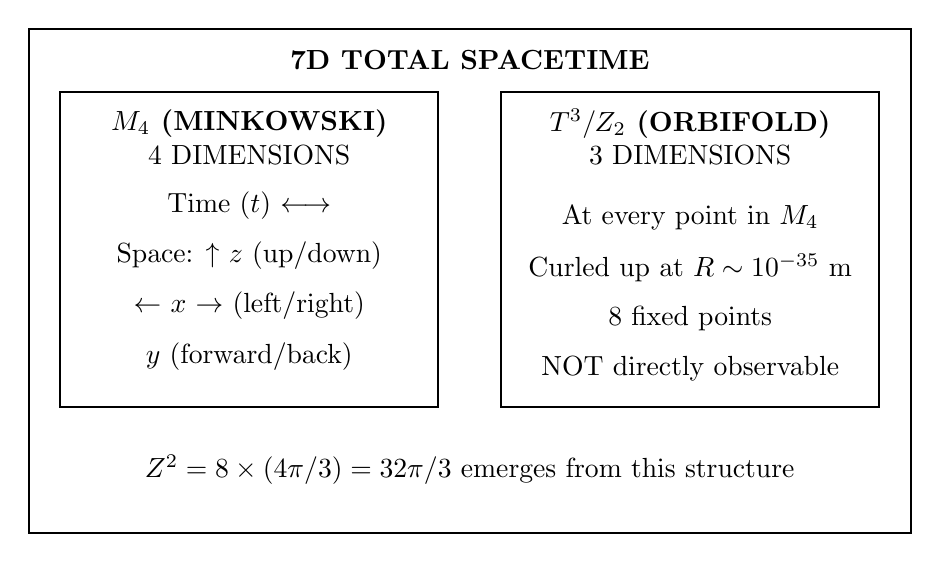
\begin{tikzpicture}[scale=0.8]
% Outer box
\draw[thick] (0,0) rectangle (14,8);
\node at (7,7.5) {\textbf{7D TOTAL SPACETIME}};

% M4 box
\draw[thick] (0.5,2) rectangle (6.5,7);
\node at (3.5,6.5) {\textbf{$M_4$ (MINKOWSKI)}};
\node at (3.5,6) {4 DIMENSIONS};
\node at (3.5,5.2) {Time $(t)$ $\longleftrightarrow$};
\node at (3.5,4.4) {Space: $\uparrow$ $z$ (up/down)};
\node at (3.5,3.6) {$\leftarrow$ $x$ $\rightarrow$ (left/right)};
\node at (3.5,2.8) {$y$ (forward/back)};

% T3/Z2 box
\draw[thick] (7.5,2) rectangle (13.5,7);
\node at (10.5,6.5) {\textbf{$T^3/Z_2$ (ORBIFOLD)}};
\node at (10.5,6) {3 DIMENSIONS};
\node at (10.5,5) {At every point in $M_4$};
\node at (10.5,4.2) {Curled up at $R \sim 10^{-35}$ m};
\node at (10.5,3.4) {8 fixed points};
\node at (10.5,2.6) {NOT directly observable};

% Bottom note
\node at (7,1) {$Z^2 = 8 \times (4\pi/3) = 32\pi/3$ emerges from this structure};
\end{tikzpicture}
\end{center}

\subsection{The Perspective Levels}

\begin{center}
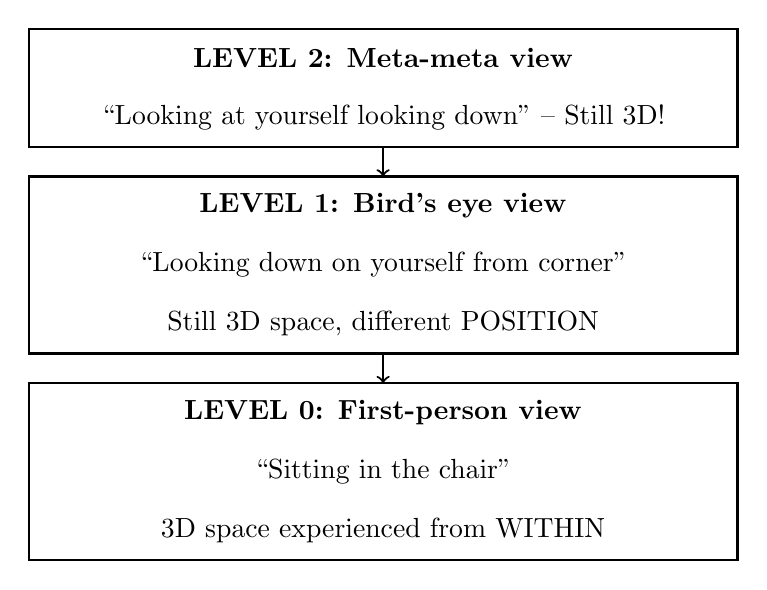
\begin{tikzpicture}[scale=0.75]
% Level 2
\draw[thick] (0,8) rectangle (12,10);
\node at (6,9.5) {\textbf{LEVEL 2: Meta-meta view}};
\node at (6,8.5) {``Looking at yourself looking down'' -- Still 3D!};

% Level 1
\draw[thick] (0,4.5) rectangle (12,7.5);
\node at (6,7) {\textbf{LEVEL 1: Bird's eye view}};
\node at (6,6) {``Looking down on yourself from corner''};
\node at (6,5) {Still 3D space, different POSITION};

% Level 0
\draw[thick] (0,1) rectangle (12,4);
\node at (6,3.5) {\textbf{LEVEL 0: First-person view}};
\node at (6,2.5) {``Sitting in the chair''};
\node at (6,1.5) {3D space experienced from WITHIN};

% Arrows
\draw[->, thick] (6,8) -- (6,7.5);
\draw[->, thick] (6,4.5) -- (6,4);
\end{tikzpicture}
\end{center}

\textbf{KEY INSIGHT:} All these ``levels'' are different VIEWPOINTS within the SAME 3D space. They are not additional spatial dimensions. They are cognitive models/representations.

\section{Where the Orbifold Actually Works}

\subsection{Domains of Applicability}

\begin{table}[h]
\centering
\begin{tabular}{@{}lll@{}}
\toprule
Domain & Applicability & Evidence \\
\midrule
Particle physics & Core domain & $\alpha^{-1}$, $\sin^2\theta_W$, generations \\
Cosmology & Core domain & $\Omega_\Lambda$, $\Omega_m$, $H_0$ \\
Galactic dynamics & Derived (via MOND) & SPARC, GN-z11 \\
Quantum gravity & Speculative & Not directly tested \\
Consciousness & Unknown & No physics connection proven \\
Everyday perception & Not applicable & Wrong scale \\
\bottomrule
\end{tabular}
\caption{Applicability of the orbifold structure.}
\end{table}

\subsection{Scale Dependence}

\begin{table}[h]
\centering
\begin{tabular}{@{}ll@{}}
\toprule
Scale & What Happens \\
\midrule
Planck ($10^{-35}$ m) & Full 7D structure relevant \\
GUT ($10^{-32}$ m) & Compactification effects, gauge unification \\
Electroweak ($10^{-18}$ m) & 4D effective theory \\
Your office chair & 4D spacetime (extra dims ``integrated out'') \\
Cosmic ($10^{26}$ m) & Cosmological parameters fixed by topology \\
\bottomrule
\end{tabular}
\caption{Scale dependence of the dimensional structure.}
\end{table}

\section{Honest Summary}

\subsection{What We Know}

\textbf{ESTABLISHED:}
\begin{enumerate}
\item We experience 3 spatial dimensions + 1 time dimension (4D)
\item Einstein's GR works in this 4D spacetime
\item The Standard Model works in this 4D spacetime
\end{enumerate}

\textbf{WELL-MOTIVATED (Z$^2$ Framework):}
\begin{enumerate}
\setcounter{enumi}{3}
\item 7D = 4D + 3D compactified might explain parameters
\item The $T^3/Z_2$ structure gives $Z^2 = 32\pi/3$
\item This predicts $\alpha^{-1} \approx 137.04$, $\sin^2\theta_W \approx 0.231$, etc.
\item Verified predictions: GN-z11, $\Omega_\Lambda$, $\Delta m^2_{31}/\Delta m^2_{21}$
\end{enumerate}

\textbf{SPECULATIVE BUT INTERESTING:}
\begin{enumerate}
\setcounter{enumi}{7}
\item Spectral dimension flow might explain MOND
\item Orbifold geometry might determine all SM parameters
\end{enumerate}

\subsection{What We Don't Know}

\begin{enumerate}
\item Whether the extra dimensions are ``real'' or just mathematical
\item Why $T^3/Z_2$ specifically (vs other compactifications)
\item How to directly detect the compactified dimensions
\item Whether this connects to consciousness at all
\item What the ``ground of reality'' actually is
\end{enumerate}

\subsection{Key Takeaways}

\begin{table}[h]
\centering
\begin{tabular}{@{}lll@{}}
\toprule
Quantity & Value & Meaning \\
\midrule
Spacetime dimensions & 7 & $M_4$ (4) + $T^3/Z_2$ (3) \\
Fixed points & 8 & Corners of fundamental domain \\
$Z^2$ & $32\pi/3$ & $8 \times (4\pi/3)$ = geometric contribution \\
$Z$ & 5.789 & $\sqrt{32\pi/3} = \sqrt{Z^2}$ \\
\bottomrule
\end{tabular}
\caption{Key dimensional quantities in the Z$^2$ framework.}
\end{table}

\textbf{There are no ``8 dimensions''---the 8 refers to fixed points.}

\vspace{1cm}
\hrule
\vspace{0.5cm}
\textit{Part of Z$^2$ Framework Research}\\
\textit{Honest Dimensional Clarification}\\
\textit{Carl Zimmerman $|$ May 2026}

\end{document}
